\section{Experimental Results \& Tests}
%Using our implementation, TRE and scan\_for\_matches, we were able to do some benchmarking in order to compare performances.
For this a virtual machine is created, using Oracle VirtualBox\footnote{virtualbox.org}. The machine running the virtualbox is running Windows 8.1 Pro x64 on an SSD, with 8,00 GB RAM, an AMD FX 4300 Quad-Core Processor 3.80 GHz, of which 1 core and 4096MB RAM was given to the virtual machine, which would run Ubuntu 14.04.2 LTS 64 bit.

We choose to test four different tools, scan\_for\_matches, TRE, Python using the Regex module and finally our own implementation. Since our implementation is focused on supporting insertion, deletion and mutation on a sequence, a simple DNA sequence $TGCAAGCGTTAAT$ with variable insertions is chosen as the search pattern. Each test was executed on a series of data files, a total of of 10 times, given an average runtime which was used in the following results.

%\begin{wrapfigure}{r}{0.6\linewidth}
%\centering
%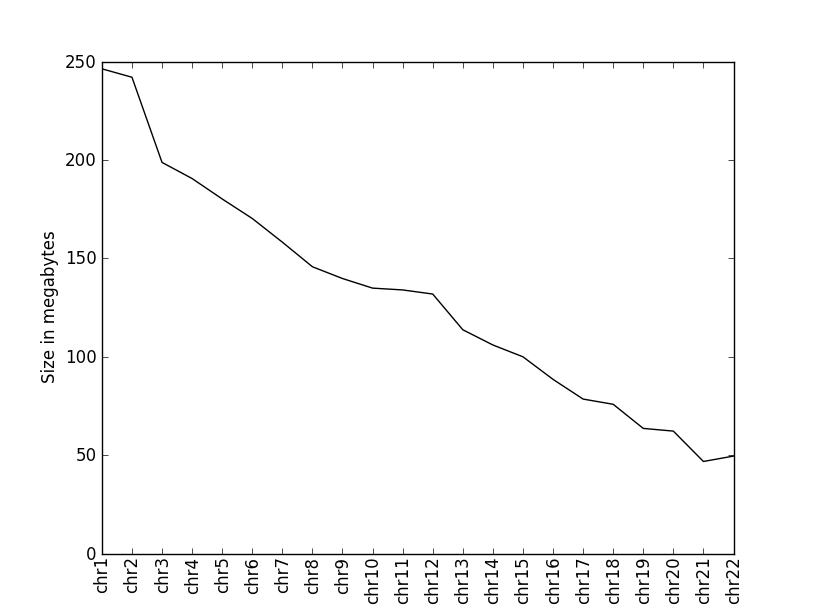
\includegraphics[width=0.6\textwidth]{Benchmarking/size.png}
%\caption{Sample files used for benchmarking, files range from 246.3 Megabytes to 46.8 Megabytes in size}
%\label{fig:size}
%\end{wrapfigure}

The testing data was selected to be in the form of the human genome chromosome sequences. Figure~\ref{fig:size} shows a series of fasta files, these files include nucleotide sequences, which all differ in size, decreasing from chr1 to chr22\footnote{http://hgdownload.cse.ucsc.edu/goldenPath/hg18/chromosomes/ JUNE 2015}. These fasta files are the kind of data which scan\_for\_matches is expected to run, and thus excellent for benchmark testing. It is worth noting however, that each of these files' lines are 50 characters long, as TRE matches through lines separately, and longer or shorter line sizes might affect the performance of TRE in running time and hits.% This was not tested however.
\begin{figure}[h!]
\centering
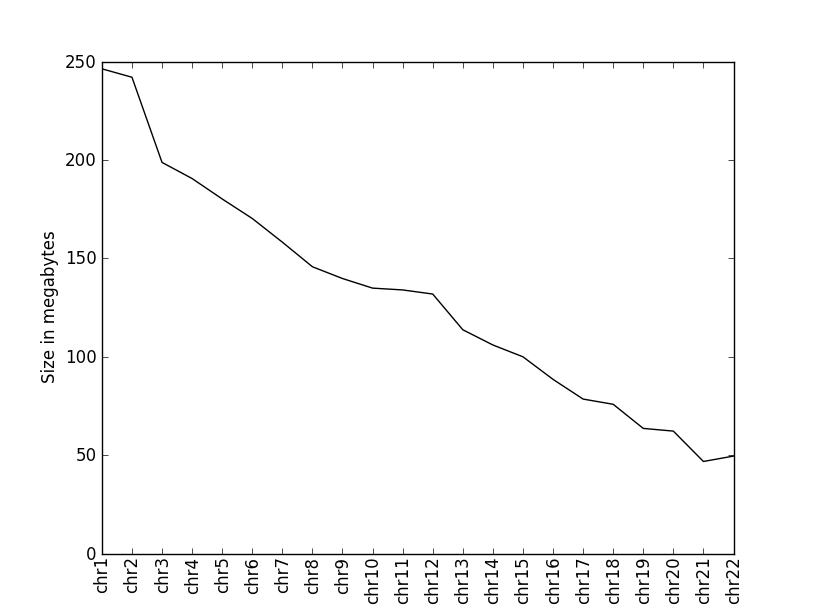
\includegraphics[width=0.7\textwidth]{Benchmarking/size.png}
\caption{Sample files used for benchmarking, files range from 246.3 Megabytes to 46.8 Megabytes in size}
\label{fig:size}
\end{figure}

\newpage

First test was to see the runtime of each program, having no mismatches in the mentioned pattern $TGCAAGCGTTAAT$. Figure~\ref{fig:0miss} displays the results, and it is evident that scan\_for\_matches is faster all the alternatives. Our implementation and python has slightly different runtime, our implementation being slightly faster, and finally TRE is the slowest tool. Common to all four tools is their decrease in runtime matches the sizes of the data files.

\begin{figure}[h!]
\centering
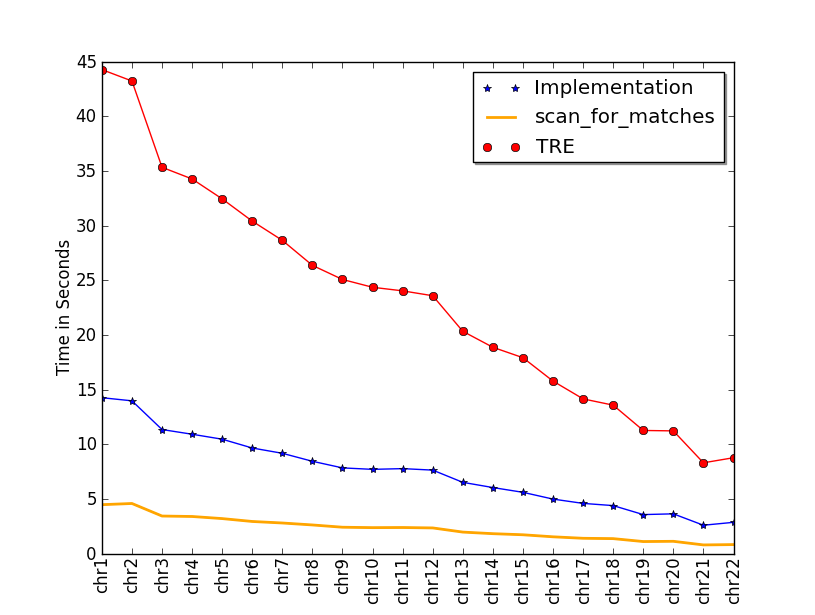
\includegraphics[width=0.7\textwidth]{Benchmarking/0miss.png}
\caption{Running time of search through fasta files mentioned in Figure~\ref{fig:size} looking for pattern TGCAAGCGTTAAT with no mismatches}
\label{fig:0miss}
\end{figure}


\begin{figure}[h!]
\centering
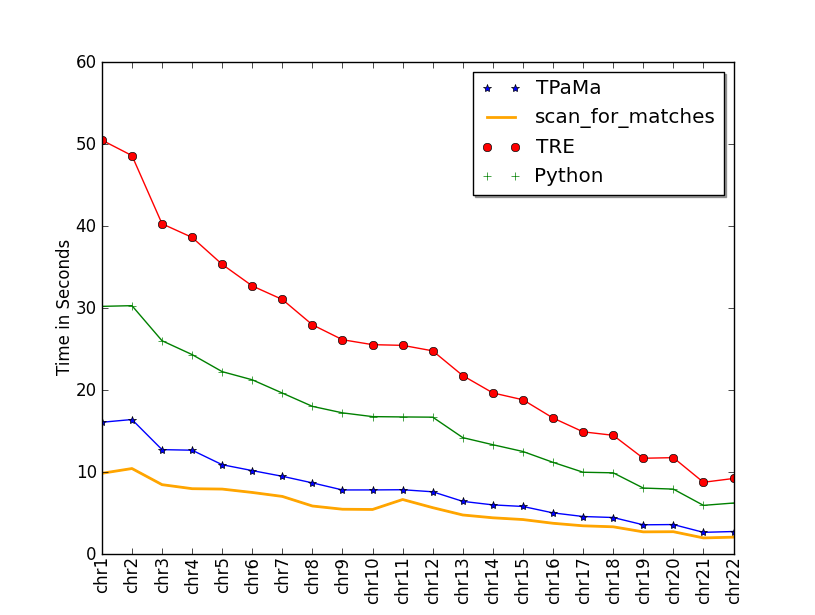
\includegraphics[width=0.7\textwidth]{Benchmarking/1ins.png}
\caption{Running time of search through fasta files mentioned in Figure~\ref{fig:size},  allowing one insertions on pattern TGCAAGCGTTAAT}
\label{fig:ins1}
\end{figure}



From Figure~\ref{fig:ins1} it is evident that there is an increase in the runtime for all four tools, scan\_for\_matches continues to be the fastest tool, while our implementation is the second fastest. Python ran at about double the speed of our implementation, and TRE continues to be the slowest tool.

\begin{figure}[h!]
\centering
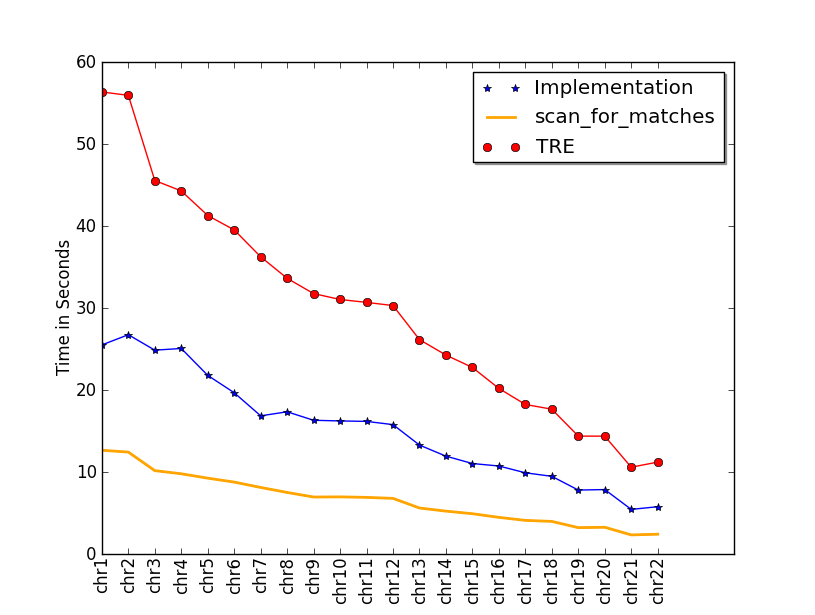
\includegraphics[width=0.7\textwidth]{Benchmarking/2ins.png}
\caption{Running time of search through fasta files mentioned in Figure~\ref{fig:size},  allowing two insertions on pattern TGCAAGCGTTAAT}
\label{fig:ins2}
\end{figure}

The next test was to see the runtime of two insertions instead of one. Looking at Figure~\ref{fig:ins2}, scan\_for\_matches did increase its runtime slightly compared to Figure~\ref{fig:ins1}, but the second insertion greatly affected our implementation, resulting in it running at about half the speed of TRE, but still faster than Python.  And while TRE also had its runtime slightly increased, it's almost unchanged from one insertion.

\begin{figure}[h!]
\centering
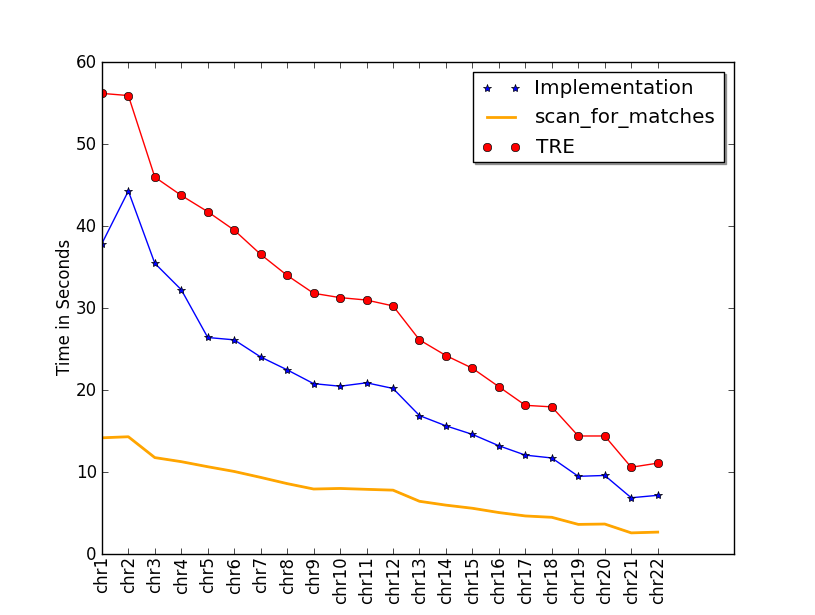
\includegraphics[width=0.7\textwidth]{Benchmarking/3ins.png}
\caption{Running time of search through fasta files mentioned in Figure~\ref{fig:size},  allowing three insertions on pattern TGCAAGCGTTAAT}
\label{fig:ins3}
\end{figure}

Testing with three insertions, Figure~\ref{fig:ins3} python is now the slowest tool, and our implementation is once again slower compared to TRE, which is now the second slowest tool, and scan\_for\_matches is still the fastest tool.

From these three tests its clear to see that our implementation has a problem with increasing number of insertions, affecting its runtime at a much higher rate than both scan\_for\_matches and TRE. It does seem, however, that Python has a similar problem. From this we can conclude that our current implementation has a major flaw, should it be used with more advanced patterns.

We suspect that flaw may be the rate of which new states are created. To test this claim, we ran our code again, on fasta file chr22.fa, measuring how the number of states, and thereby the amount of work needed to pattern-match, relates to the number of mismatches allowed.

\begin{figure}[h!]
\centering
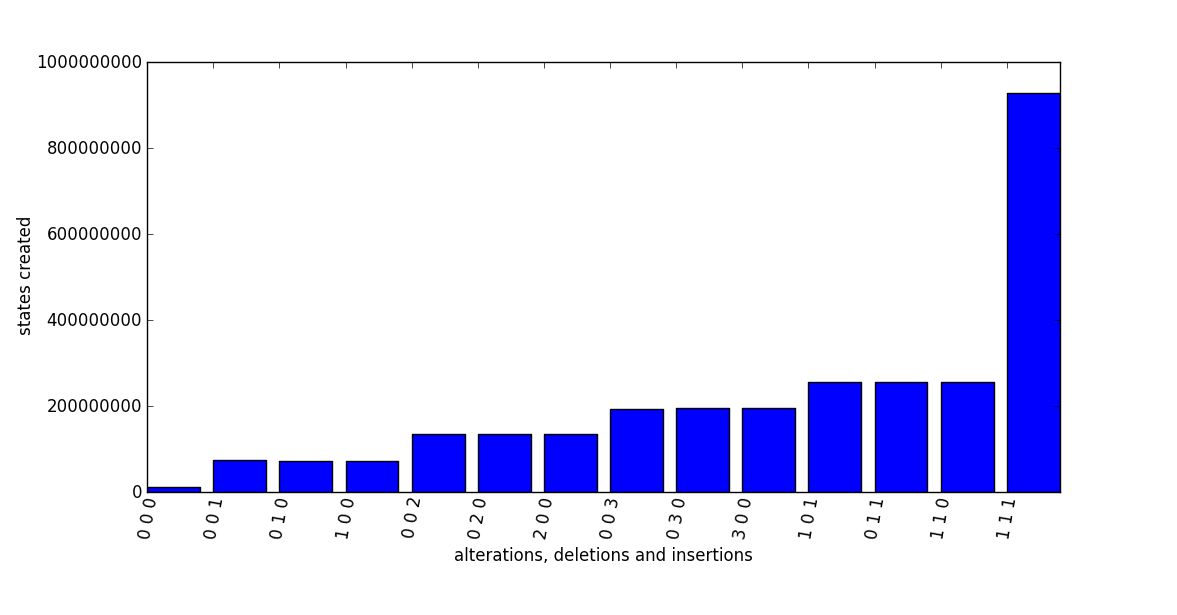
\includegraphics[width=0.9\textwidth]{Benchmarking/states_graph.png}
\caption{Bar chart showcasing the number of states created corresponding to the number of mismatches allowed.}
\label{fig:statesgraph}
\end{figure}

The chart in Figure~\ref{fig:statesgraph} displays an increasing number of states, corresponding to the increasing number of mismatches. We can observe how allowing any number of mismatches of the same type, be it insertion, alternation or deletion, yields roughly the same number of states, actually deletions and alternations gives exactly the same amount of states, as their behavior is exactly the same.

Another observation is how two mismatches of different types result in more new states than two or even three mismatches of the same kind would. This can be explained due to the implementation creating two new states every time a mismatch is encountered in the data. Causing an exponential growth of states, opposed a linear growth. Finally there is a measurement with a mismatch of every kind, causing a massive growth in states, once again being due to an exponential growth, now making three states per mismatch, instead of two or one.  


Another interesting thing to test for was the number of hits when searching the files, in table~\ref{tab:hits} the number of hits which came up when searching on file chr1.fa are shown.

\begin{table}[h!]
\centering
\begin{tabular}{ l | c c r }
& 1 insertion & 2 insertions & 3 insertions\\
\hline
Our implementation& 5 &  48 & 235 \\
TRE& 1 & 19 & 76 \\
scan\_for\_matches & 5 & 43  & 192 \\
Python & 5 & 48 & 235
\end{tabular}
\caption{Number of hits in fasta file chr1, using the mentioned benchmark tests.}
\label{tab:hits}
\end{table}

The primary reason that our implementation gets more results than scan\_for\_matches is that our implementation finds every single match in the file, including overlapping matches, while scan\_for\_matches, by default, only finds matches which do not overlap. TRE has the major disadvantage here that it does not match across newlines, causing it to miss a lot of matches. Finally Python has the same amount of matches as our implementation.